\documentclass{standalone}
\usepackage{tikz}
\usepackage{standalone}
\begin{document}
	
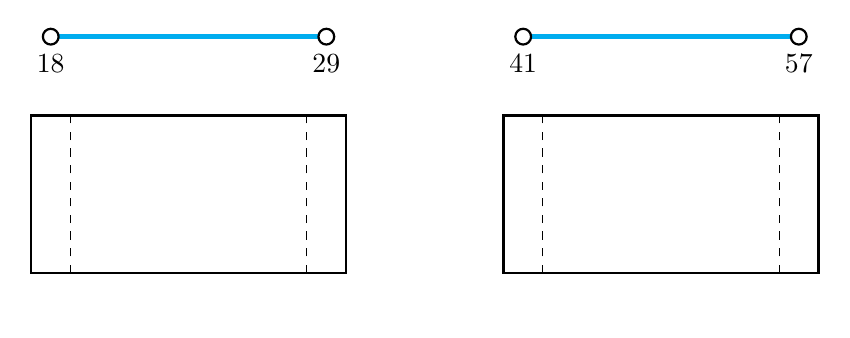
\begin{tikzpicture}
%\draw [help lines] (-1,-2) grid (11,5);

\draw [cyan, ultra thick] (0.25,3) -- (3.75,3);
\draw [cyan, ultra thick] (6.25,3) -- (9.75,3);



\draw [fill=white, thick] (0.25,3) circle [radius = 0.1];
\draw [fill=white, thick] (3.75,3) circle [radius = 0.1];
\draw [fill=white, thick] (6.25,3) circle [radius = 0.1];
\draw [fill=white, thick] (9.75,3) circle [radius = 0.1];


\draw [thick] (0,0) rectangle (4,2);
\draw [thick] (6,0) rectangle (10,2);

\draw [dashed] (0.5,0) -- (0.5,2);
\draw [dashed] (3.5,0) -- (3.5,2);

\draw [dashed] (6.5,0) -- (6.5,2);
\draw [dashed] (9.5,0) -- (9.5,2);

\node [below] at (0.25,2.9) {18};
\node [below] at (3.75,2.9) {29};
\node [below] at (6.25,2.9) {41};
\node [below] at (9.75,2.9) {57};

\node [below] at (0.25,0) {\textcolor{white}{18}};
\node [below] at (3.75,0) {\textcolor{white}{29}};
\node [below] at (6.25,0) {\textcolor{white}{41}};
\node [below] at (9.75,0) {\textcolor{white}{57}};



\end{tikzpicture}
	
\end{document}